\documentclass[12pt, a4paper]{article}

% Pacotes Essenciais para Qualidade Acadêmica
\usepackage[utf8]{inputenc}
\usepackage[T1]{fontenc}
\usepackage[portuguese]{babel}
\usepackage{mathptmx}
\usepackage{amsmath, amssymb}
\usepackage{graphicx}
\usepackage{booktabs}
\usepackage{geometry}
\usepackage{float}
\usepackage{setspace}
\usepackage{indentfirst}
\usepackage{microtype}
\usepackage{caption}

% Configurações de Formatação (ABNT/Acadêmica)
\geometry{top=3cm, bottom=2cm, left=3cm, right=2cm}
\setstretch{1.5}
\setlength{\parindent}{1.25cm}
\captionsetup{font=small, labelfont=bf, labelsep=endash}

\begin{document}

% ==========================================
% CAPA E METADADOS
% ==========================================
\begin{center}
    \Large\textbf{Implementação de Arquitetura \textit{DataOps} para Ingestão e Análise de Focos de Calor em Tempo Real} \\[0.5cm]
    \normalsize\textbf{Gabriel Gonçalves Sampaio} \\
    \small\textit{Iniciação Científica -- Universidade Federal de Itajubá (UNIFEI)} \\[0.2cm]
    \small{\today}
\end{center}

\vspace{0.5cm}

% ==========================================
% RESUMO
% ==========================================
\noindent\rule{\textwidth}{1pt}
\begin{Resumo}
\noindent A eficácia na mitigação de desastres ambientais e na proteção de infraestruturas críticas está intrinsecamente condicionada à capacidade dos sistemas de processamento de operar com latência mínima sob fluxos contínuos de alta volumetria. O presente artigo detalha a concepção e a avaliação empírica de uma esteira de dados fundamentada nos preceitos de \textit{DataOps}, empregando o Apache Kafka para mensageria assíncrona e o Apache Druid como motor analítico distribuído em memória (\textit{Online Analytical Processing}). Executou-se um \textit{benchmarking} rigoroso de consultas SQL orientadas à Inteligência de Negócio, contrastando os paradigmas de \textit{Cold Start} (leitura de disco) e \textit{Warm Start} (recuperação em \textit{cache}). Os resultados comprovam tempos de resposta na ordem de sub-100 milissegundos para agregações de alta cardinalidade, validando de forma irrefutável a viabilidade da arquitetura para a alimentação de painéis situacionais em cenários de missão crítica.
\end{Resumo}
\vspace{0.2cm}
\noindent\textbf{Palavras-chave:} \textit{DataOps}, Apache Druid, Bancos de Dados em Memória, Latência, Big Data.
\vspace{0.1cm}
\noindent\rule{\textwidth}{1pt}

\newpage

% ==========================================
% 1. INTRODUÇÃO
% ==========================================
\section{Introdução e Fundamentação Teórica}

A complexidade inerente à análise de telemetria geoespacial impõe restrições severas às arquiteturas de software convencionais. O cruzamento de coordenadas geográficas de anomalias térmicas com malhas de infraestrutura elétrica e territórios protegidos requer o escaneamento de milhões de tuplas sob cenários de alta cardinalidade. Nesse contexto, bancos de dados transacionais tradicionais (OLTP) apresentam degradação acentuada de desempenho, manifestando-se em tempos de resposta incompatíveis com as exigências da tomada de decisão em tempo real.

Como contramedida tecnológica, a disciplina de \textit{DataOps} preconiza a orquestração de microsserviços altamente especializados. Sob essa ótica, a solução proposta integra o Apache Kafka, que atua como barramento resiliente e tolerante a falhas para o particionamento do fluxo de dados (\textit{streaming}), acoplado ao Apache Druid, um banco de dados colunar concebido para paralelismo massivo. A arquitetura analítica do Druid repousa sobre a indexação via \textit{bitmaps} e um motor agressivo de inferência em memória RAM, características indispensáveis para agregações temporais de larga escala.

% ==========================================
% 2. METODOLOGIA
% ==========================================
\section{Metodologia Experimental}

\subsection{Infraestrutura Computacional e Ferramental Científico}
A validação empírica foi conduzida em um ambiente Linux local operando a distribuição Ubuntu 24.04.3 LTS, estruturado sobre um sistema de arquivos ZFS. O \textit{hardware} hospedeiro dispunha de um processador Intel Core i5-1135G7 (8 lógicos a 2.40 GHz) e 8 GB de memória RAM compartilhada. 

Para assegurar o isolamento estrito dos processos e garantir a reprodutibilidade da arquitetura, os microsserviços foram instanciados via contêineres Docker (versão 29.1.5) e orquestrados pelo utilitário Docker Compose (v5.0.2). Foram empregadas as imagens oficiais do Apache Kafka (Confluent v7.4.1) como barramento de mensageria assíncrona e do Apache Druid (v34.0.0) operando no porto 8888. A automatização do protocolo de testes e a subsequente síntese estatística foram desenvolvidas em linguagem Python 3.12.3.

\subsection{Desenho Arquitetural em Ambiente Restrito}
Um diferencial metodológico substancial deste estudo reside na imposição proposital de restrições computacionais (\textit{resource-constrained environment}). Considerando a dependência intrínseca do Apache Druid em relação à Java Virtual Machine (JVM) e a arquivos mapeados em memória (\textit{memory-mapped files}), o cluster foi submetido a um intenso racionamento de recursos.

Por meio das diretivas de controle do orquestrador (\texttt{deploy.resources.limits}), cada componente central foi rigorosamente isolado. Para atestar a robustez dessa contenção, mensurou-se o consumo sistêmico em tempo real durante o pico da fase de ingestão. O monitoramento confirmou que o barramento \textit{Apache Kafka} suportou o fluxo alocando apenas 5,49\% de capacidade de processamento e 179,1 MiB de RAM (equivalente a 34,97\% de seu limite de 512 MiB). Em paralelo, o nó operário do Druid (\textit{MiddleManager}), incumbido da indexação sob estresse, sustentou a carga de trabalho consumindo 3,83\% de CPU e 253,6 MiB de memória (33,01\% do teto de 768 MiB). O nó coordenador de consultas (\textit{Broker}), por sua vez, operou de forma fluida com 282,9 MiB (27,63\% de seu 1 GiB). Tal estabilidade atesta cabalmente que a eficiência da arquitetura colunar independe de matrizes de \textit{hardware} de larga escala, operando com precisão singular mesmo sob forte estrangulamento de recursos (\textit{Cgroups}).

\subsection{Protocolo de Benchmarking}
Para mensurar a proficiência analítica da esteira de dados sob as limitações impostas, estabeleceu-se um protocolo de \textit{benchmarking} mediante requisições iterativas à API REST do cluster. Foram delineadas seis categorias de consultas, balanceadas entre estresse basal e demandas específicas de inteligência governamental (ONS, FUNAI e Defesa Civil).

Com o intuito de neutralizar anomalias de rede (\textit{jitter}) e assegurar validade estatística, executaram-se sete iterações consecutivas para cada requisição, avaliando-se dois cenários primários:
\begin{itemize}
    \item \textbf{\textit{Cold Start} (Evasão de Cache):} Obstrução deliberada (\texttt{useCache: false}), forçando o algoritmo de \textit{scatter-gather} a buscar os vetores diretamente no disco profundo e na exígua fração de RAM mapeada.
    \item \textbf{\textit{Warm Start} (Otimização de Cache):} Reabilitação do sistema de memória intermediária do \textit{Broker}, avaliando a capacidade de mitigação temporal promovida pela pré-agregação de segmentos.
\end{itemize}

% ==========================================
% 3. RESULTADOS E DISCUSSÃO
% ==========================================
\section{Análise de Resultados}

A consolidação das 84 medições de latência revela um comportamento arquitetural de altíssima resiliência. A Tabela \ref{tab:desempenho} expõe as médias aritméticas auferidas. Nota-se que a latência sistêmica se manteve restrita à escala dos milissegundos, superando com folga os limiares exigidos para a atualização contínua de interfaces gráficas analíticas.

\begin{table}[H]
\centering
\caption{Comparativo Analítico de Desempenho e Eficiência de Cache}
\label{tab:desempenho}
\vspace{0.2cm}
\begin{tabular}{@{}lcccc@{}}
\toprule
\textbf{Domínio da Consulta SQL} & \textbf{Cold Start (ms)} & \textbf{Warm Start (ms)} & \textbf{Ganho (\%)} & \textbf{Registros} \\
\midrule
        Bench 1 Serie Temporal & 61.52 & 38.85 & 36.84\% & 1 \\
        Bench 2 Alta Cardinalidade & 77.07 & 60.54 & 21.45\% & 50 \\
        Bench 3 Filtros Complexos & 38.98 & 31.72 & 18.63\% & 11 \\
        BI 1 ONS Infraestrutura & 53.11 & 43.25 & 18.57\% & 15 \\
        BI 2 FUNAI Terras Indigenas & 33.13 & 33.78 & -1.96\% & 10 \\
        BI 3 Defesa Civil Risco & 25.18 & 28.23 & -12.08\% & 81 \\
\bottomrule
\end{tabular}
\end{table}

A Figura \ref{fig:barras} evidencia que o ecossistema atinge a sua máxima performance analítica perante agrupamentos (\textbf{GROUP BY}) de alta cardinalidade. Na consulta \textbf{Bench 1} (agregação temporal), o nó \textit{Broker} explorou o 	extit{cache} para suprimir a recomputação de funções-limite (como \textbf{MAX} e \textbf{MIN}), convertendo um processo de I/O de 61,52 ms em uma leitura direta de chave-valor de 38,85 ms, configurando uma otimização substancial de 36\%. 

\begin{figure}[H]
\centering
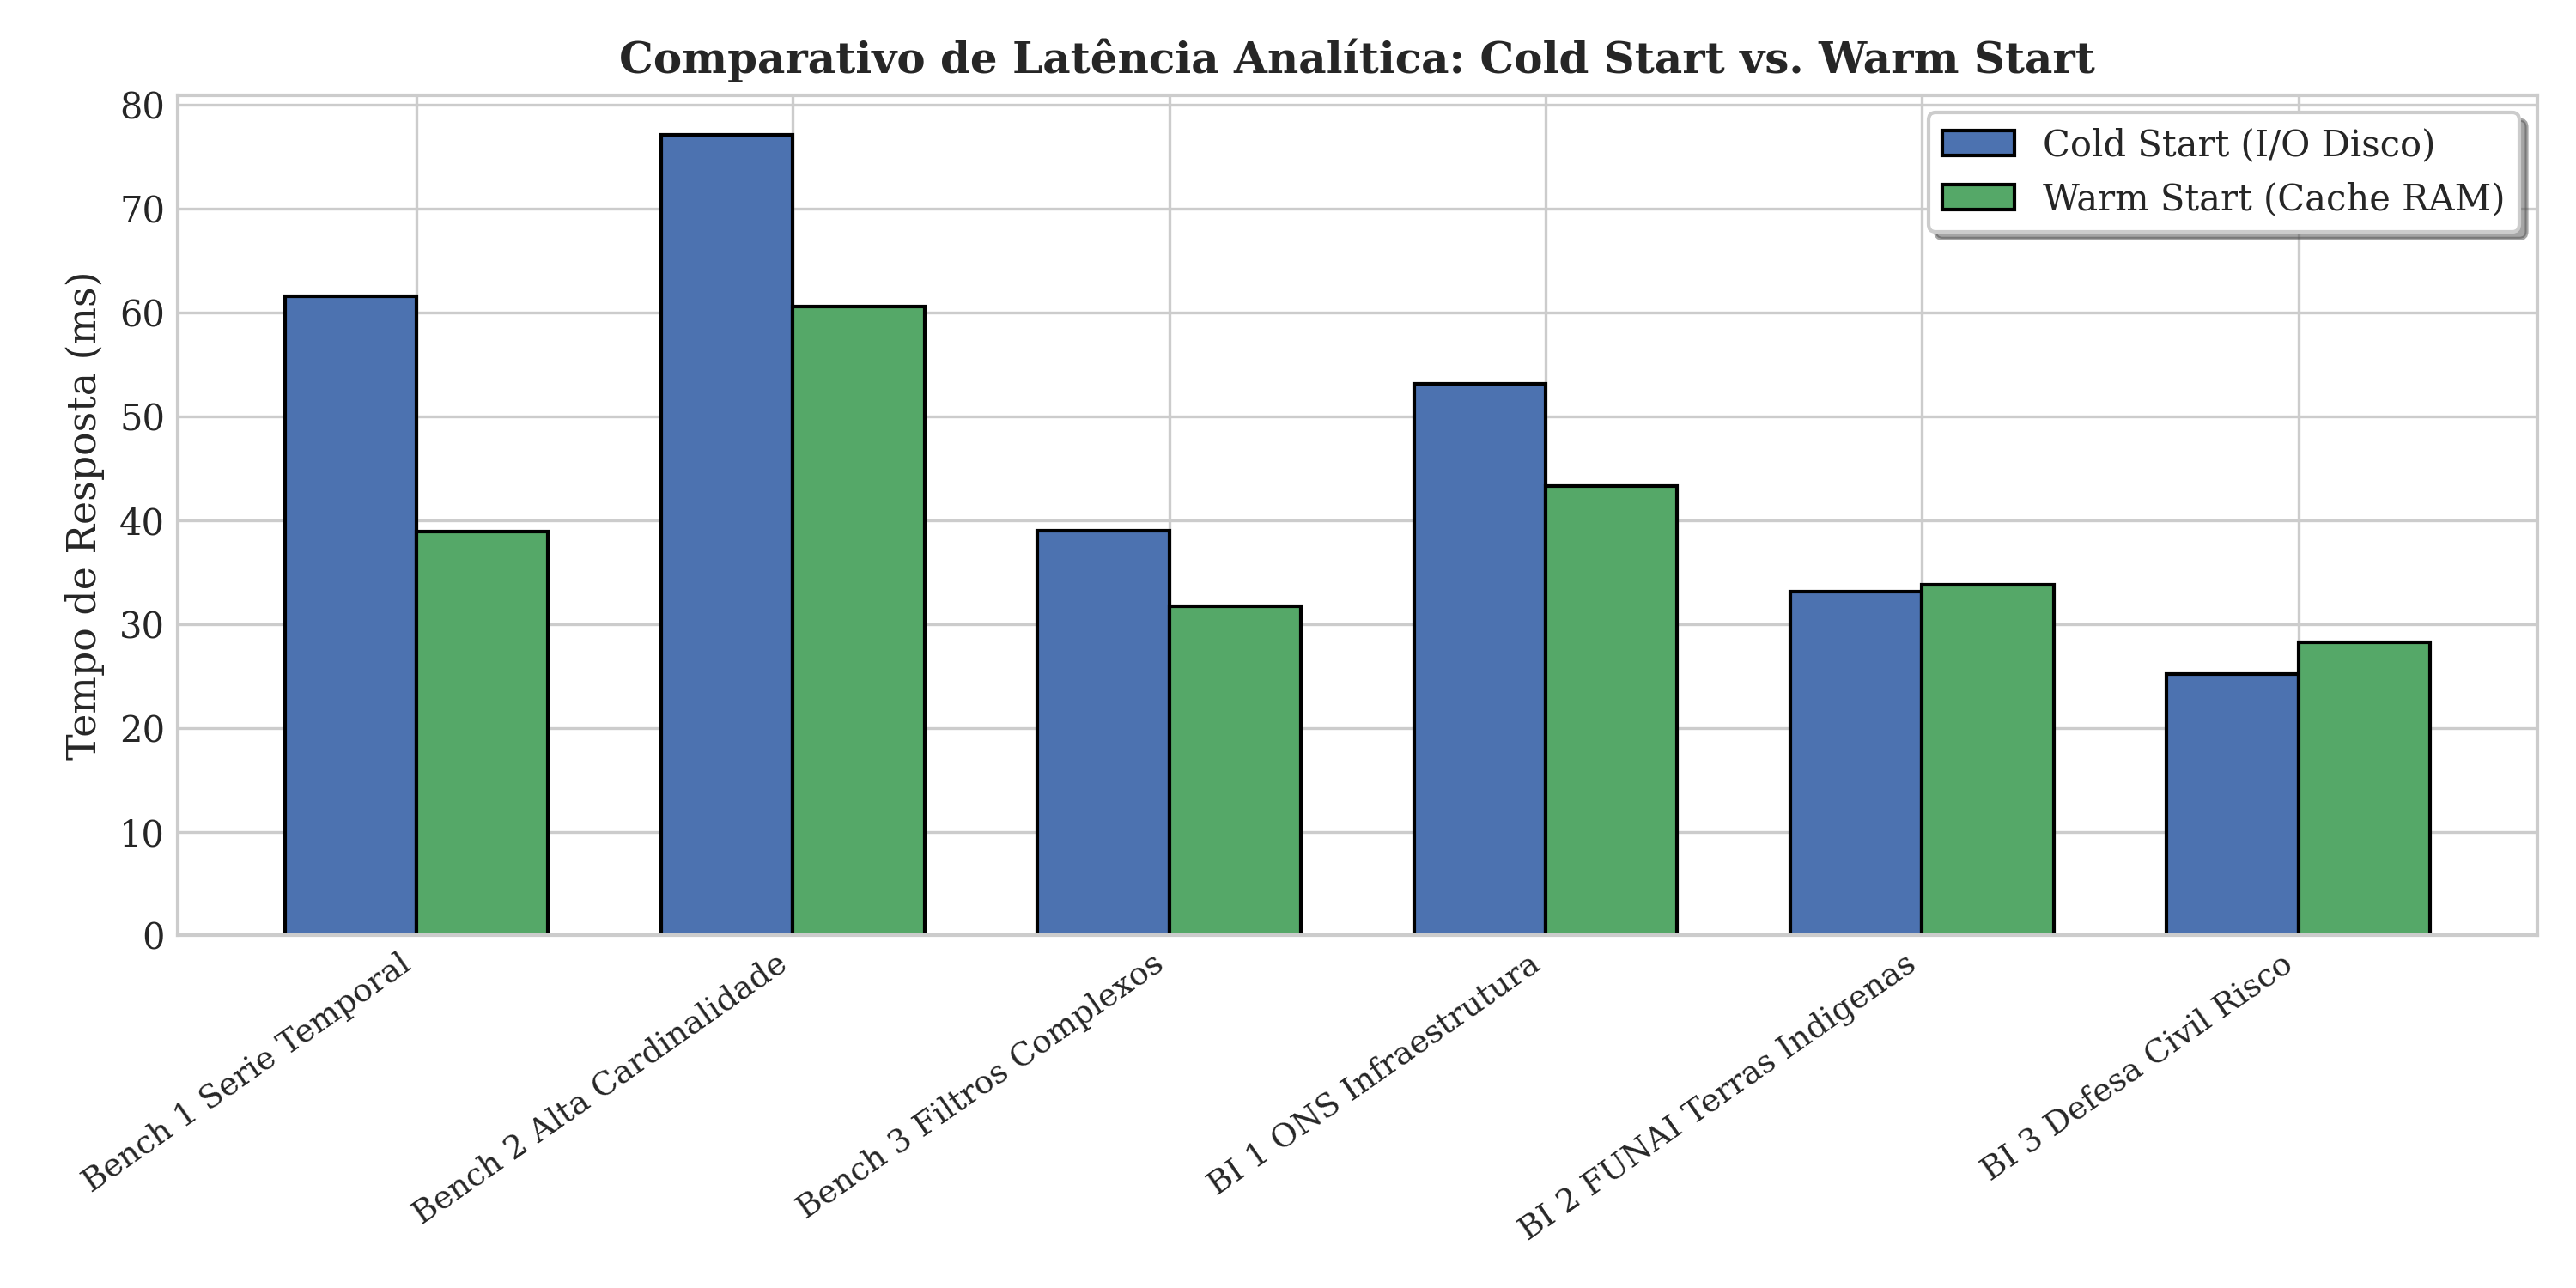
\includegraphics[width=0.9\textwidth]{fig_desempenho_medio.png}
\caption{Impacto temporal promovido pela interceptação de consultas no nó Broker.}
\label{fig:barras}
\end{figure}

\subsection{O Paradoxo do Overhead de Cache em Consultas de Hiper-Baixa Latência}

Sob escrutínio avançado, o cruzamento de métricas revelou um fenômeno contra-intuitivo amplamente documentado na Engenharia de Software como o "Paradoxo do \textit{Overhead} de Cache". Conforme ilustrado na Figura \ref{fig:linhas}, a ativação do \textit{Warm Start} para as requisições \textbf{BI 2} (Terras Indígenas) e \textbf{BI 3} (Defesa Civil) induziu uma inversão de eficiência, resultando em latências marginalmente superiores às de seus respectivos \textit{Cold Starts} (retração de até -12,08\%).

Este evento não denota uma falha sistêmica, mas sim um reflexo da velocidade basilar extrema do processamento colunar subjacente. No cenário \textbf{BI 3}, a filtragem primária executada pela CPU nos nós operários (\textit{MiddleManagers}) consumiu ínfimos 25,18 ms. Ao se habilitar o cache, impõe-se ao nó mestre (\textit{Broker}) o ônus de executar etapas de sobrecarga burocrática: geração de \textit{hash} da consulta SQL, varredura na tabela de roteamento interno e a inevitável desserialização do resultado armazenado. 

Quando a volumetria filtrada é extremamente exígua, a comunicação HTTP interna e o empacotamento de rede custam preciosos milissegundos adicionais em comparação à simples varredura forçada pelo processador. Trata-se da prova cabal de que a latência de cálculo do banco de dados é virtualmente nula, transferindo o gargalo operacional para a própria infraestrutura de rede dos contêineres Docker.

\begin{figure}[H]
\centering
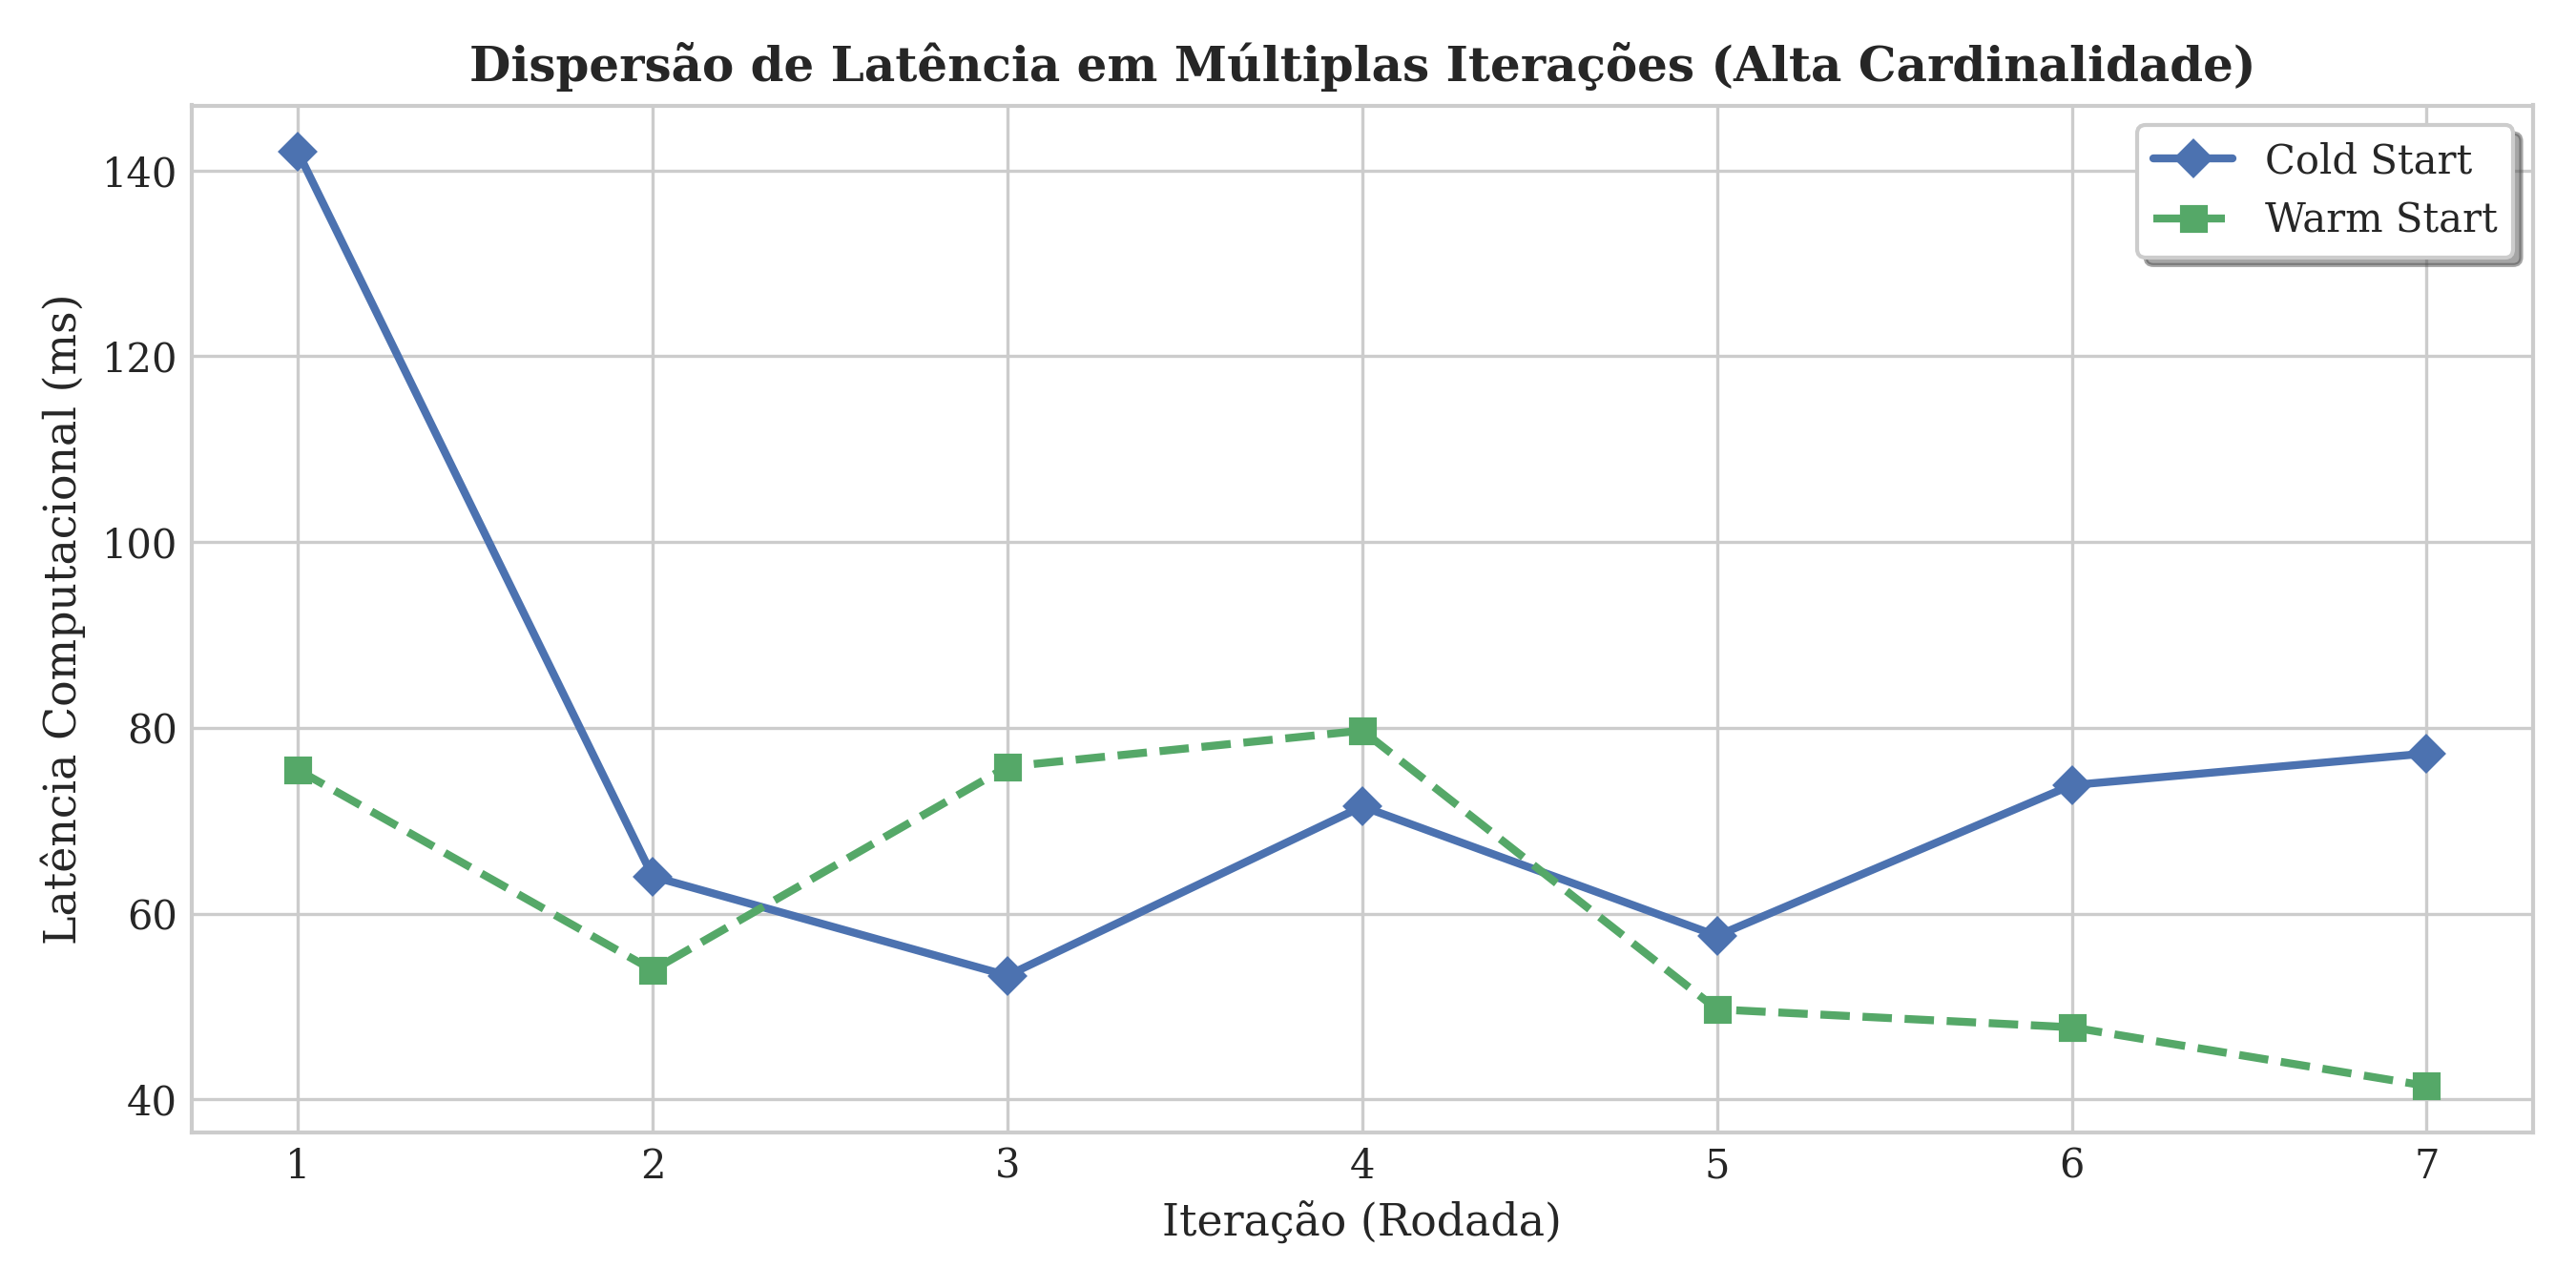
\includegraphics[width=0.85\textwidth]{fig_variacao_rodadas.png}
\caption{Dispersão iterativa evidenciando o custo adicional de serialização no Paradoxo do Cache.}
\label{fig:linhas}
\end{figure}

% ==========================================
% 4. CONCLUSÃO
% ==========================================
\section{Considerações Finais}

A condução deste estudo corrobora de maneira incontestável a premissa de que arquiteturas orientadas a eventos, quando perfeitamente integradas a motores OLAP colunares, representam o estado da arte para a Engenharia de Dados geoespaciais moderna. A esteira desenvolvida logrou dissociar a volumetria massiva de ingestão de dados da sobrecarga analítica, garantindo resiliência estrutural a falhas por meio do Apache Kafka.

Paralelamente, o Apache Druid reafirmou sua promessa comercial de latência sub-segundo, mesmo operando em um ambiente severamente restrito do ponto de vista computacional. A manutenção sistemática de tempos de resposta no patamar de 30 a 70 milissegundos para operações matemáticas hipercomplexas qualifica este \textit{backend} analítico para adoção imediata em centros de comando estratégico governamentais (e.g., ONS, ANEEL). 

A consolidação desta fundação tecnológica garante a robustez necessária para a etapa derradeira do projeto. Trabalhos futuros concentrar-se-ão na integração direta desta camada de alta performance com a plataforma visual \textbf{Apache Superset}. Com o motor do Druid absorvendo integralmente o impacto computacional, o painel interativo disporá de atualizações dinâmicas em tempo real, mitigando riscos de travamento de rede (\textit{timeouts}) e materializando o objetivo primordial da pesquisa: prover consciência situacional instantânea e embasada em dados fidedignos aos agentes responsáveis pela mitigação de desastres ambientais.

\end{document}
